\documentclass[runningheads]{llncs}

\usepackage{graphicx}
\usepackage{listings}
\usepackage{xcolor}
\usepackage{subfig}


\definecolor{mGreen}{rgb}{0,0.6,0}
\definecolor{mGray}{rgb}{0.5,0.5,0.5}
\definecolor{mPurple}{rgb}{0.58,0,0.82}
\definecolor{backgroundColour}{rgb}{0.95,0.95,0.92}

\lstdefinestyle{CStyle}{
    backgroundcolor=\color{backgroundColour},   
    commentstyle=\color{mGreen},
    keywordstyle=\color{magenta},
    numberstyle=\tiny\color{mGray},
    stringstyle=\color{mPurple},
    basicstyle=\footnotesize,
    breakatwhitespace=false,         
    breaklines=true,                 
    captionpos=b,                    
    keepspaces=true,                 
    numbers=left,                    
    numbersep=5pt,                  
    showspaces=false,                
    showstringspaces=false,
    showtabs=false,                  
    tabsize=2,
    language=C
}

\begin{document}
%
\title{Behavioral Biometric Classifier on 8051 Microcontroller\thanks{Supported by CSEN 702: Microprocessors Course}}

\author{Abdullah Elkady \and Mohamed Ibrahim \and Amr Kayid \and Ahmed Shawky \and Ahmed Sabek}


\institute{German University in Cairo, Egypt \\
\email{\{abdullah.elkady, mohamed.meeza, amr.kayid, \\
ahmed.ahmedhussein, ahmed.sabek\}@guc.edu.eg}}

\authorrunning{A. Elkady \and M. Ibrahim \and A. Kayid \and A. Shawky \and A. Sabek}

\maketitle             


\begin{abstract}
A simple behavioral biometric classifier on 8051 Microcontroller that can identify users based on their keystroke dynamics profiles. Implemented using C language on Keil C51 development tool.

\keywords{Behavioral Biometric  \and Classifier \and Microcontroller \and Dwell time \and Flight time.}
\end{abstract}

%
%
%

\section{Introduction}
\subsection{behavioral biometric}
In this project we used the behavioral biometric of Keystroke Dynamics to identify an individual's character typing profile on a keyboard or keypad. The keystroke rhythms of a user are measured to develop a unique biometric profile of the user's typing pattern for future authentication, the project idea is similar to the one that was used by Coursera~\cite{ref_article1} for verifying learners before submitting graded quizzes and assignments. \newline \newline \newline

Keystroke dynamics can therefore be described as a software-based algorithm that measures both dwell and flight time to authenticate identity. where dwell time is the duration that a key is pressed, while flight time is the duration between keystrokes. \newline \newline \newline \newline \newline

\subsection{Project Idea:} 
This project is divided into two phases, traning and testing phase. \\

In the training phase, the participants are asked to enter a certain word \textbf{".tie5Ronal"} \underline{5 times}, then during the training, the average flight time of each character in the word is calculated, taking the average of the 5 trails, a unique profile is created for each participant which will be used to verify the user in the testing phase. \\

In the testing phase, one of the participant will be selected randomly and will be asked to enter the same passcode ".tie5Ronal", then our implementation measures the distance between the test vector and the saved profiles and identify the user's identity based on the shortest distance between the two vectors, using the Euclidean metric. \newline \newline \newline

%
%
%

\section{Implementation}

\subsection{Brief Description}
Our implementation starts with initializing and setting the serial port for 2400 baud at 12MHz, and enabling mode 1 (8-bit UART) to enable receiver, along with enabling the interrupts for T0 and the global interrupts. \newline \newline 

After the initialization phase, we continuously check for training and testing phases by checking on \textbf{P1.1}. If we are in the training phase, we check for which user profile (\textit{A or B}) will be trained, then the training phase starts for the selected user using the following functions 

\begin{lstlisting}[style=CStyle]
void trainUser(unsigned int timings[])
\end{lstlisting}

This function calculate the total training time for the user in the 5 attempts,
the function calculate the time of each keystroke usign the following function
\begin{lstlisting}[style=CStyle]
unsigned char *calculateTimings()
\end{lstlisting}
after 5 successful attempts of input runs, we average the resulting time and save it in the user's profile. \newline \newline 

In the testing phase, a user is selected randomly and asked to enter the same passcode,
then we calculate the timing of the user, and using the Euclidean Distance Algorithm in the following function
\begin{lstlisting}[style=CStyle]
unsigned int calculateEculidean(unsigned int timings[])
\end{lstlisting}
we determine the users identity by the closest vector in the saved profile. \newline


\subsection{Team Work}

The code was divided into several steps and functions as follows:
\begin{itemize}
  \setlength\itemsep{2em}

\item \textbf{\textit{Serial port Setup and Initialization}}
\begin{lstlisting}[style=CStyle]
void init()
\end{lstlisting}


\item \textbf{\textit{Time Setup and Calculations}}
\begin{lstlisting}[style=CStyle]
void resetTimer()
void stopTimer()
void handleOverflow(void) interrupt 1
\end{lstlisting}


\item \textbf{\textit{Training Phase}}
\begin{lstlisting}[style=CStyle]
void trainUser(unsigned int timings[])
\end{lstlisting}


\item \textbf{\textit{Similarity Calculations }}
\begin{lstlisting}[style=CStyle]
unsigned int calculateEculidean(unsigned int timings[])
\end{lstlisting}

\item \textbf{\textit{Testing Phase}}
\begin{lstlisting}[style=CStyle]
unsigned char *calculateTimings()
void flashLED(void)
\end{lstlisting}
\end{itemize}


The work was distributed among the team members equally and they worked together to combine the final functions and testing the final version of the system.

\newpage

%
%
%

\section{User Guide}

Our System starts with checking on \textbf{P1} \\
then we start by training two user \textbf{\textit{(A \& B)}}, as indicated in the following two figures.

\begin{figure}%
    \centering
    \subfloat[User A]{{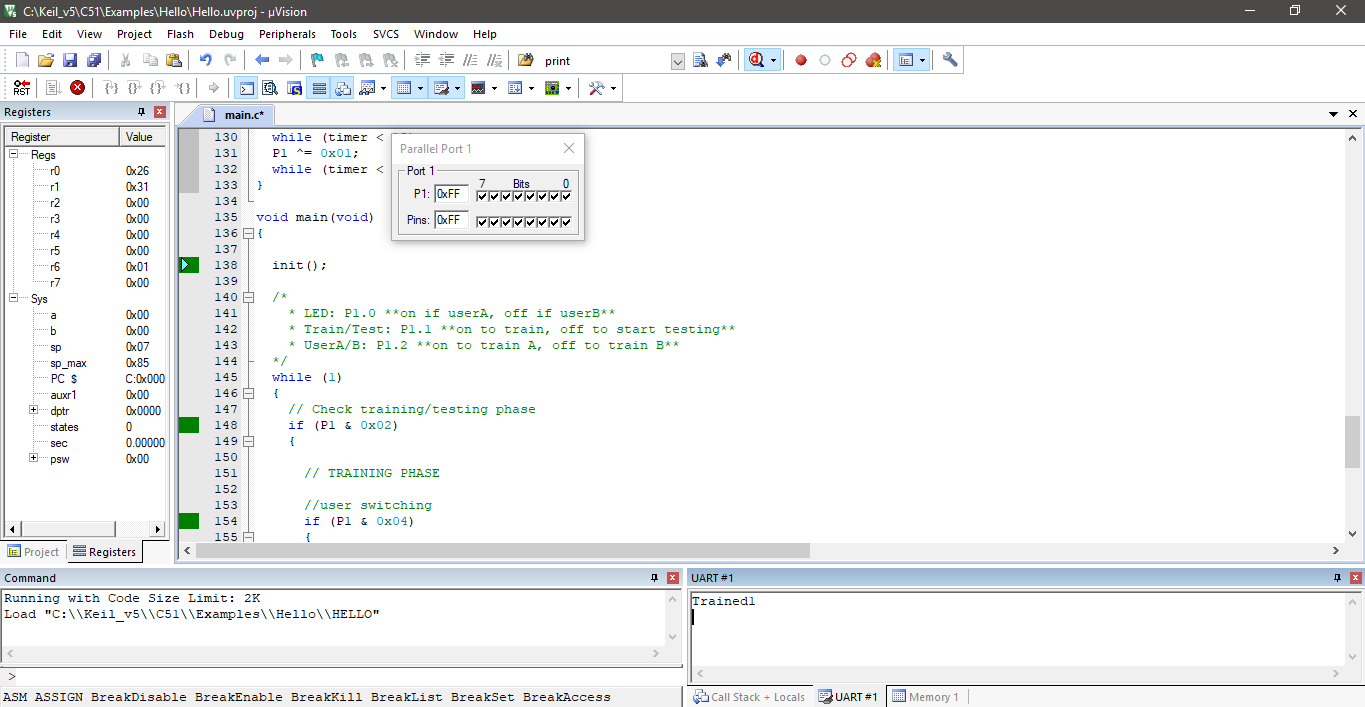
\includegraphics[width=5cm]{TrianingUserA.png} }}%
    \qquad
    \subfloat[User B]{{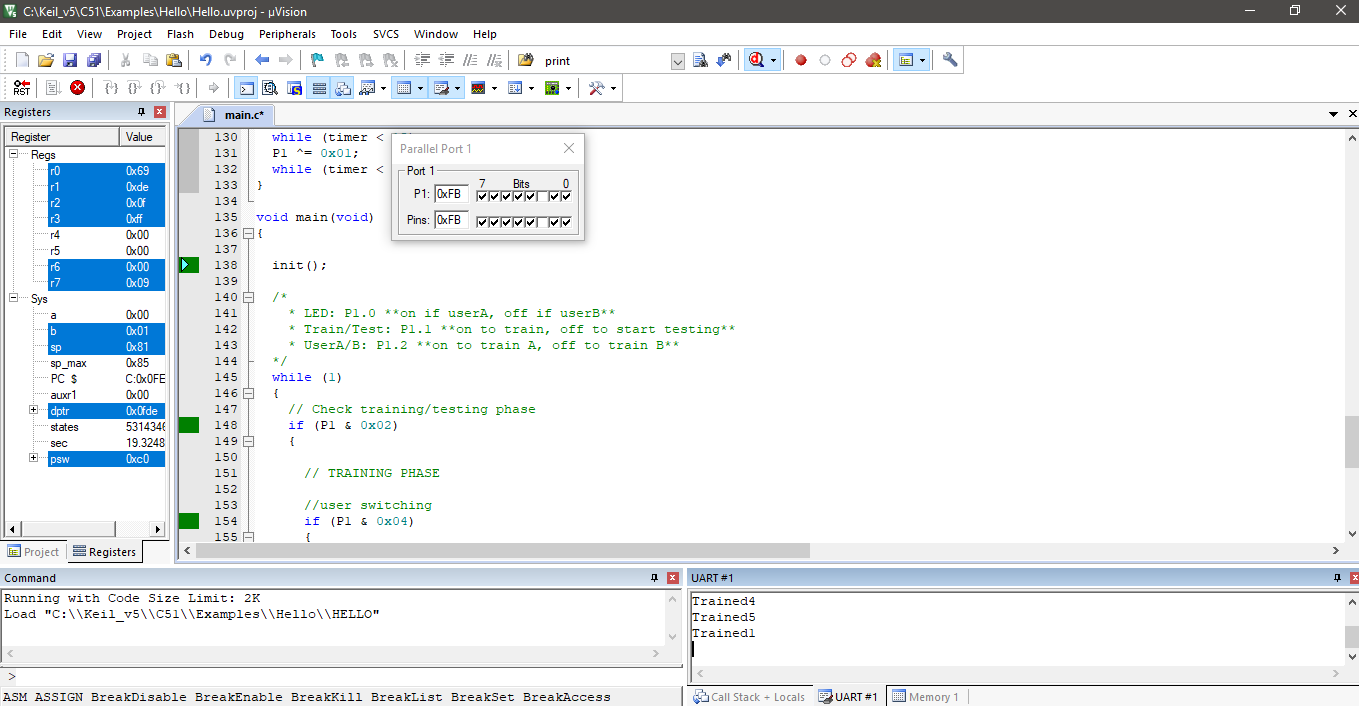
\includegraphics[width=5cm]{TrianingUserB.png} }}%
    \caption{Training User A \& B}%
    \label{fig:example}%
\end{figure}

After the training is done, we start the testing phase and the system is able to indicated which user is using the system now as indicated in the following figure.


\begin{figure}%
    \centering
    \subfloat[Testing]{{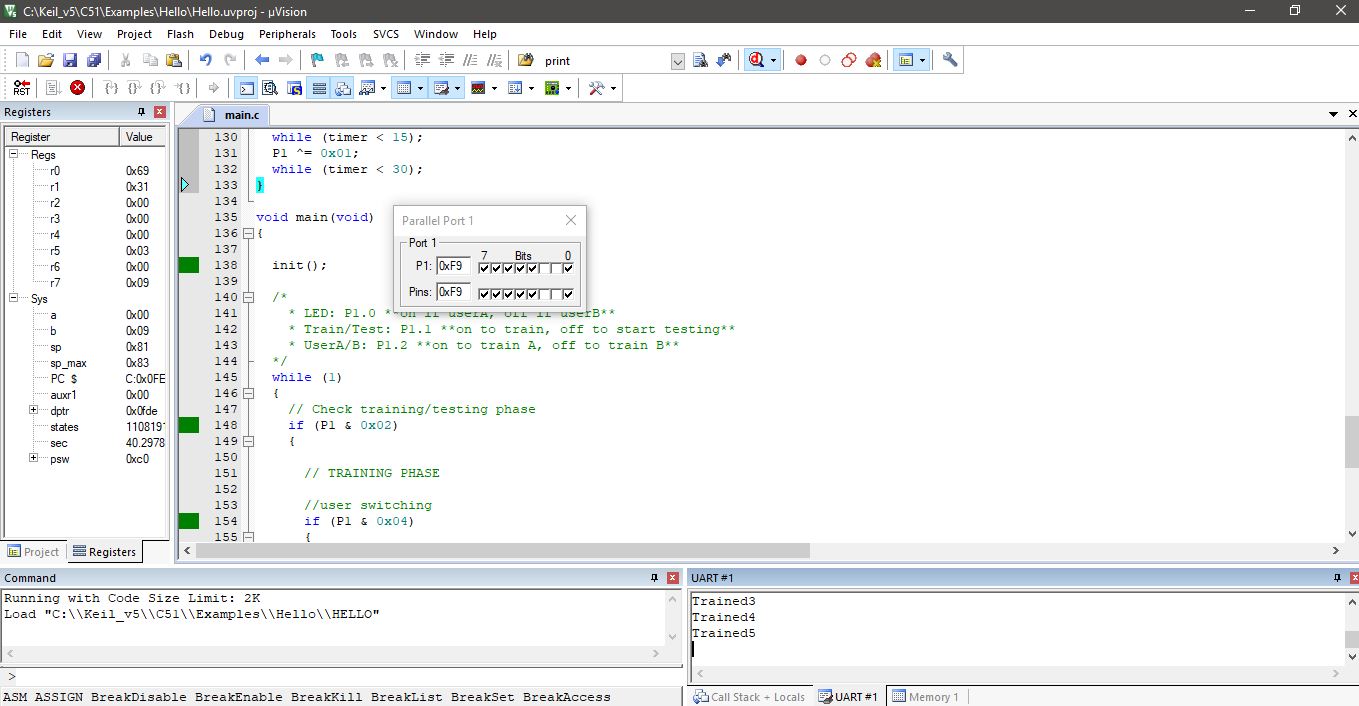
\includegraphics[width=10cm]{Testing.png} }}%
    \qquad
    % \subfloat[label 2]{{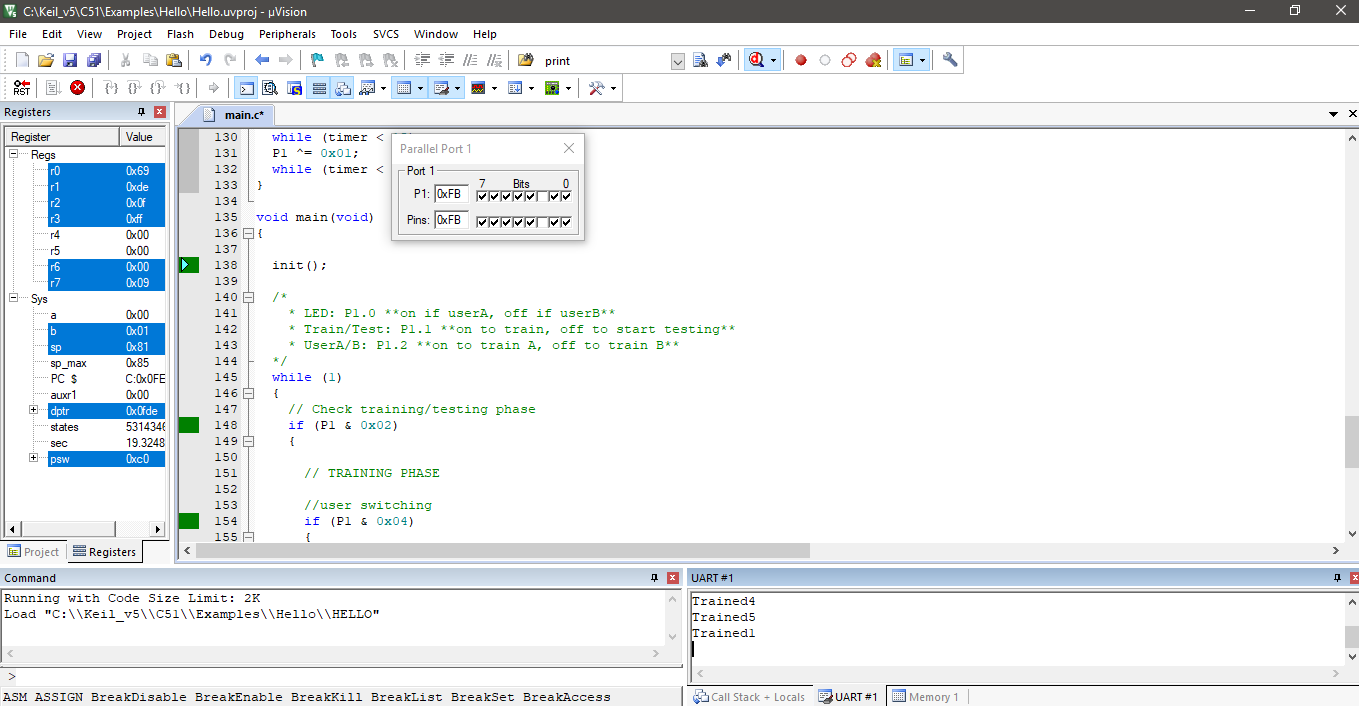
\includegraphics[width=5cm]{TrianingUserB.png} }}%
    \caption{Testing Phase}%
    \label{fig:example}%
\end{figure}

\newpage

%
%
%

\section{Results}

Results Results Results Results Results Results Results Results Results Results Results Results Results Results Results Results Results Results Results Results Results Results Results Results Results Results Results Results Results Results Results Results Results Results Results Results Results Results Results Results Results Results Results Results Results Results Results Results Results Results Results Results Results Results Results Results Results Results Results Results Results Results Results Results Results Results Results Results Results Results Results Results Results Results Results Results Results Results Results Results Results Results Results Results Results Results Results Results Results Results Results Results Results Results Results Results Results Results Results Results Results Results Results Results Results Results Results Results Results Results Results Results Results Results Results Results Results Results Results Results Results Results Results Results Results Results Results Results Results Results Results Results Results Results Results Results Results Results Results Results Results Results Results Results Results Results Results Results Results Results Results Results Results Results Results Results Results Results Results Results Results Results Results Results Results Results Results Results Results Results Results Results Results Results Results Results Results Results Results Results Results Results Results Results Results Results Results Results Results Results Results Results Results Results Results Results Results Results Results Results Results Results Results Results Results Results Results Results Results Results Results Results Results Results Results Results Results Results Results Results Results Results Results Results Results Results Results Results Results Results Results Results Results Results 

%
% ---- Bibliography ----
%
% BibTeX users should specify bibliography style 'splncs04'.
% References will then be sorted and formatted in the correct style.
%
% \bibliographystyle{splncs04}
% \bibliography{mybibliography}
%
\begin{thebibliography}{8}
\bibitem{ref_article1}
Ng, A.: Ubiquity symposium: MOOCs and technology to advance learning and learning research: offering verified credentials in massive open online courses. ACM

\end{thebibliography}
\end{document}
